\section{Тестирование}
\label{sec:test}

Работа агента проверена диалогом с системой в пользовательском интерфейсе NIKA. Контрольные сущности выбраны так, чтобы были представлены оба случая: заметка отсутствует в локальной БЗ (требуется обогащение из Википедии) и заметка уже есть (обогащение пропускается).

Сценарий тестирования приведён в таблице~\ref{tab:tests}. В третьем столбце указано, выполнялось ли обращение к внешнему источнику; в последнем~\mdash  ожидаемое начало ответа системы (фраза строится шаблоном <<имя~--- заметка>>).

\begin{table}[H]
	\centering
	\scriptsize
	\begin{tabular}{|p{3.6cm}|p{2.3cm}|p{2.6cm}|p{5.9cm}|}
		\hline
		Сообщение & Сущность & Обращение к Википедии & Ответ в интерфейсе NIKA (начало) \\
		\hline
		Что такое Thriller? & \texttt{thriller\_album} & да: статья <<Thriller>> & Thriller~--- шестой студийный альбом американского музыканта Майкла Джексона \ldots \\
		\hline
		Что такое Bohemian Rhapsody? & \texttt{bohemian\_rhapsody} & нет: \texttt{nrel\_note} есть в БЗ & Bohemian Rhapsody~--- песня группы Queen (1975) из альбома A Night at the Opera \ldots \\
		\hline
		Что такое Волшебная флейта? & \texttt{the\_magic\_flute} & да: статья <<Волшебная флейта>> & Волшебная флейта~--- опера-зингшпиль Моцарта в 2-х действиях \ldots \\
		\hline
		Что такое The Dark Side of the Moon? & \texttt{the\_dark\_side\newline\_of\_the\_moon} & да: статья <<The Dark Side of the Moon>> & The Dark Side of the Moon~--- восьмой студийный альбом британской рок-группы Pink Floyd \ldots \\
		\hline
		Что исполнил Thriller? & \texttt{thriller\_album} & нет: заметка уже погружена & Thriller~--- шестой студийный альбом \ldots (повторное обращение пропущено) \\
		\hline
	\end{tabular}
	\caption{Тестирование агента обогащения сущностей}
	\label{tab:tests}
\end{table}

Диалог пользователя с системой зафиксирован в пользовательском интерфейсе NIKA (рисунок~\ref{fig:dialog}).

\IfFileExists{png/dialog-enrichment.png}{%
\begin{figure}[H]
	\centering
	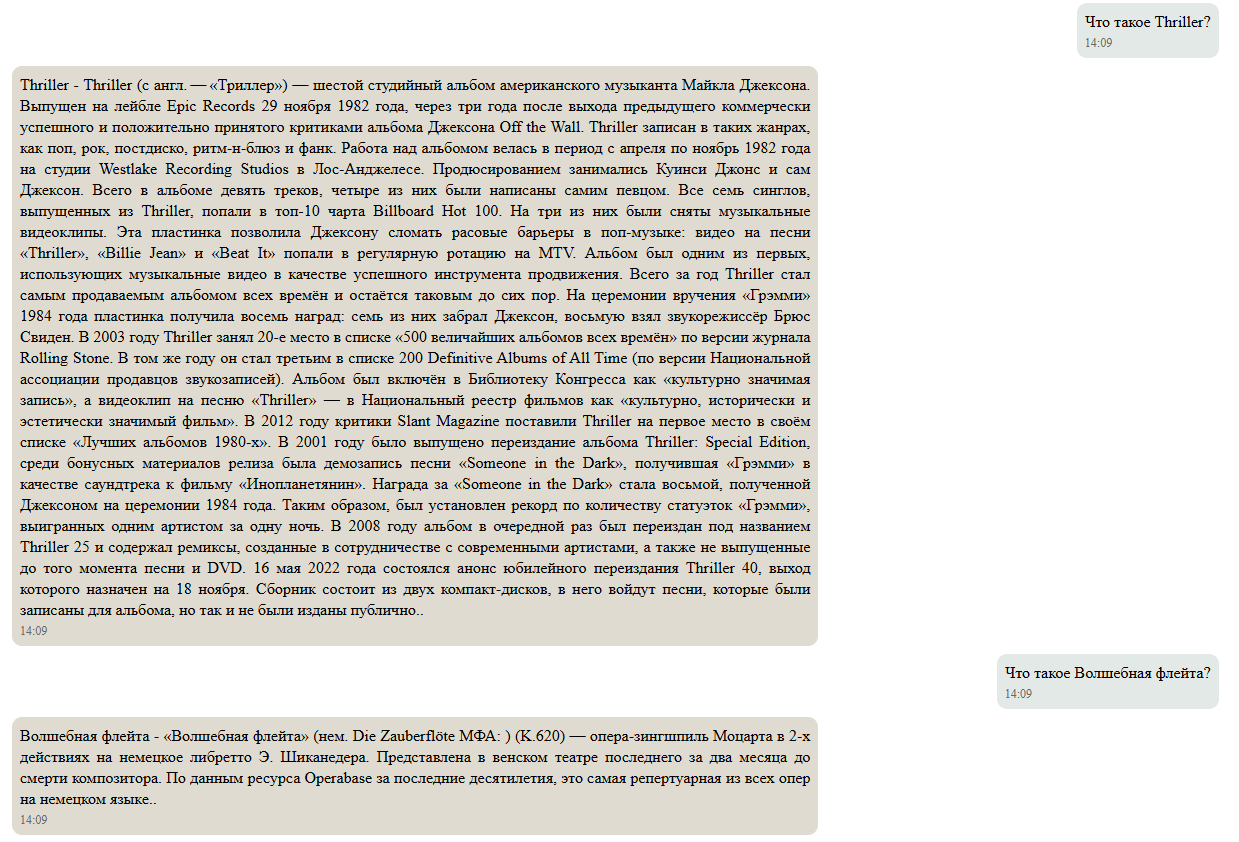
\includegraphics[width=\textwidth]{dialog-enrichment}
	\caption{Диалог обогащения сущностей в интерфейсе NIKA}
	\label{fig:dialog}
\end{figure}
}{%
\begin{figure}[H]
	\centering
	\fbox{\parbox{0.9\textwidth}{\centering\vspace{2em}
	Скриншот диалога (файл \texttt{png/dialog-enrichment.png})\\добавляется после сборки отчёта.\vspace{2em}}}
	\caption{Диалог обогащения сущностей в интерфейсе NIKA}
	\label{fig:dialog}
\end{figure}
}

Работа агента подтверждена журналами системы: в журнале problem-solver видны шаги <<enriching music entity from Wikipedia>> и <<Trying to generate by formula: lr\_message\_about\_entity>>, в журнале py-sc-server~\mdash  <<Searching Wikipedia for: Thriller>>, <<Found Wikipedia page: Thriller>>, <<Entity enriched successfully>>. Повторный вопрос к уже обогащенной сущности вызывает пропуск обогащения: агент фиксирует наличие \texttt{nrel\_note} и сразу передаёт управление построению ответа.
